\documentclass[11pt]{article}
\input{headers4}

\usepackage{fancyhdr} 
\usepackage{tikz}  
\pagestyle{fancy}      
\lhead{MA453 Spring 2018 - Homework 4}               
\rhead{Harris Christiansen (christih@purdue.edu)}

\usepackage{mathrsfs}
\usepackage[strict]{changepage}  

\begin{document}

\title{Homework 4}
\date{p77 F.1, p78 H.1, p86 A.1 (a,b,c), A.2 (b,c,d), and A.4 (d)}
\maketitle

\thispagestyle{fancy}
\pagestyle{fancy}

\begin{enumerate}

%%% Problem 1: p77 F.1
\item {\bfseries p77 F.1.} Let $G$ be the group of symmetries of the regular hexagon. List the elements of $G$ (there are 12 of them).
	\begin{center}
	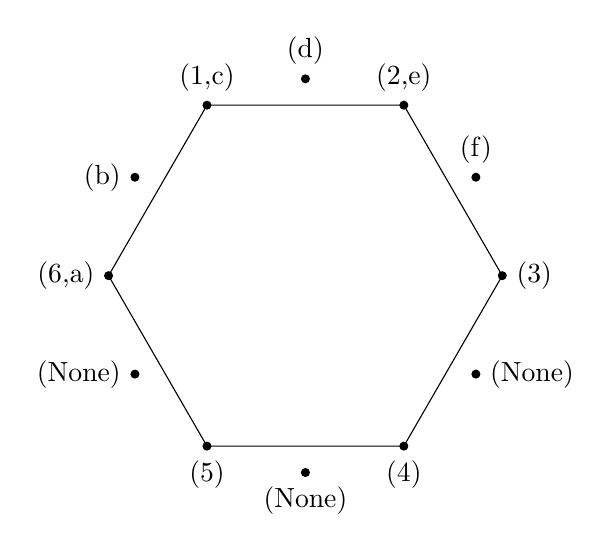
\begin{tikzpicture}
		\newdimen\R
		\R=2.5cm
		\draw (0:\R) \foreach \x in {60,120,...,360} {  -- (\x:\R) };
		\foreach \x/\l/\p in
		{
		30/{(f)}/above,
		60/{(2,e)}/above,
		90/{(d)}/above,
		120/{(1,c)}/above,
		150/{(b)}/left,
		180/{(6,a)}/left,
		210/{(None)}/left,
		240/{(5)}/below,
		270/{(None)}/below,
		300/{(4)}/below,
		330/{(None)}/right,
		360/{(3)}/right
		}
		\node[inner sep=1pt,circle,draw,fill,label={\p:\l}] at (\x:\R) {};
	\end{tikzpicture}
	\end{center}

	(No need to write the group table of $G$.)
  
	{\bfseries Solution.}
	
	$R_0 = \begin{pmatrix}
		1 & 2 & 3 & 4 & 5 & 6 \\
		1 & 2 & 3 & 4 & 5 & 6
	\end{pmatrix}$
	$R_1 = \begin{pmatrix}
		1 & 2 & 3 & 4 & 5 & 6 \\
		2 & 3 & 4 & 5 & 6 & 1
	\end{pmatrix}$
	$R_2 = \begin{pmatrix}
		1 & 2 & 3 & 4 & 5 & 6 \\
		3 & 4 & 5 & 6 & 1 & 2
	\end{pmatrix}$
	
	$R_3 = \begin{pmatrix}
		1 & 2 & 3 & 4 & 5 & 6 \\
		4 & 5 & 6 & 1 & 2 & 3
	\end{pmatrix}$
	$R_4 = \begin{pmatrix}
		1 & 2 & 3 & 4 & 5 & 6 \\
		5 & 6 & 1 & 2 & 3 & 4
	\end{pmatrix}$
	$R_5 = \begin{pmatrix}
		1 & 2 & 3 & 4 & 5 & 6 \\
		6 & 1 & 2 & 3 & 4 & 5
	\end{pmatrix}$
	
	$R_6 = \begin{pmatrix}
		1 & 2 & 3 & 4 & 5 & 6 \\
		6 & 5 & 4 & 3 & 2 & 1
	\end{pmatrix}$
	$R_7 = \begin{pmatrix}
		1 & 2 & 3 & 4 & 5 & 6 \\
		5 & 4 & 3 & 2 & 1 & 6
	\end{pmatrix}$
	$R_8 = \begin{pmatrix}
		1 & 2 & 3 & 4 & 5 & 6 \\
		4 & 3 & 2 & 1 & 6 & 5
	\end{pmatrix}$
	
	$R_9 = \begin{pmatrix}
		1 & 2 & 3 & 4 & 5 & 6 \\
		3 & 2 & 1 & 6 & 5 & 4
	\end{pmatrix}$
	$R_{10} = \begin{pmatrix}
		1 & 2 & 3 & 4 & 5 & 6 \\
		2 & 1 & 6 & 5 & 4 & 3
	\end{pmatrix}$
	$R_{11} = \begin{pmatrix}
		1 & 2 & 3 & 4 & 5 & 6 \\
		1 & 6 & 5 & 4 & 3 & 2
	\end{pmatrix}$

%%% Problem 2: p78 H.1
\item {\bfseries p78 H.1.} Let $A$ be a set of $a \in A$. Let $G$ be the subset of $S_A$ consisting of all the permutation $F$ of $A$ such that $F(a) = a$. Prove that $G$ is a subgroup of $S_A$.
  
	{\bfseries Solution.}
	
	\begin{proof}
	To prove $G$ is a subgroup of $S_A$, we must show:
	
	\begin{itemize}
	\item if $f \in S$ then $f^{-1} \in S$ \\
	Because $F(a)$ is the identity permutation, it follows that $F^{-1}F(a) = F(a) = a$. Thus, it is closed under inverses.
	
	\item if $f,g \in S$ then $fg \in S$ \\
	Because $F(a) = a \forall a \in S_A$, then $\forall f,g \in G \rightarrow fg(a) = f(g(a)) = f(a) = a$. Thus, it is closed under multiplication.
	\end{itemize}
	
	Thus, $G$ is a subgroup of $S_A$.
	
	\end{proof}
  
\newpage

%%% Problem 3: p86 A.1 (a,b,c)
\item {\bfseries p86 A.1 (a,b,c).} Compute each of the following products in $S_9$. (Write your answer as a singular permutation.)
  
	{\bfseries Solution.}
	
	\begin{enumerate}
  
		\item (145)(37)(682) =
		$\begin{pmatrix}
			1 & 2 & 3 & 4 & 5 & 6 & 7 & 8 & 9 \\
			4 & 6 & 7 & 5 & 1 & 8 & 3 & 2 & 9
		\end{pmatrix}$
		
		\item (17)(628)(9354) =
		$\begin{pmatrix}
			1 & 2 & 3 & 4 & 5 & 6 & 7 & 8 & 9 \\
			7 & 8 & 5 & 9 & 4 & 2 & 1 & 6 & 3
		\end{pmatrix}$
		
		\item (71825)(36)(49) =
		$\begin{pmatrix}
			1 & 2 & 3 & 4 & 5 & 6 & 7 & 8 & 9 \\
			8 & 5 & 6 & 9 & 7 & 3 & 1 & 2 & 4
		\end{pmatrix}$
  
  \end{enumerate}

%%% Problem 4: p86 A.2 (b,c,d)
\item {\bfseries p86 A.2 (b,c,d).} Write each of the following permutations in $S_9$ as a product of disjoint cycles:
  
	{\bfseries Solution.}
	
	\begin{enumerate}
	
		\item Not Assigned
	
		\item 
		$\begin{pmatrix}
			1 & 2 & 3 & 4 & 5 & 6 & 7 & 8 & 9 \\
			7 & 4 & 9 & 2 & 3 & 8 & 1 & 6 & 5
		\end{pmatrix}$
		= (17)(24)(395)(68)
		
		\item 
		$\begin{pmatrix}
			1 & 2 & 3 & 4 & 5 & 6 & 7 & 8 & 9 \\
			7 & 9 & 5 & 3 & 1 & 2 & 4 & 8 & 6
		\end{pmatrix}$
		= (17435)(296)
		
		\item 
		$\begin{pmatrix}
			1 & 2 & 3 & 4 & 5 & 6 & 7 & 8 & 9 \\
			9 & 8 & 7 & 4 & 3 & 6 & 5 & 1 & 2
		\end{pmatrix}$
		= (1928)(375)
  
  \end{enumerate}

%%% Problem 5: p86 A.4 (d)
\item {\bfseries p86 A.4 (d).} If $\alpha = (3714), \beta = (123), and \gamma = (24135)$ in $S_7$, express each of the following as a product of disjoint cycles:

	(d) $\beta^2\alpha\gamma$
  
	{\bfseries Solution.}
  	
  	\begin{align*}
		\beta^2 \alpha \gamma &= (123)(123)(3714)(24135) \\
		&= (132)(3714)(24135) \\
		&= (17)(243)(24135) \\
		&= (173452) \\
	\end{align*}
	
\newpage

\end{enumerate}

\end{document}
